% Pseudospectra of the 64x64 Jordan block. Generated by a short script.
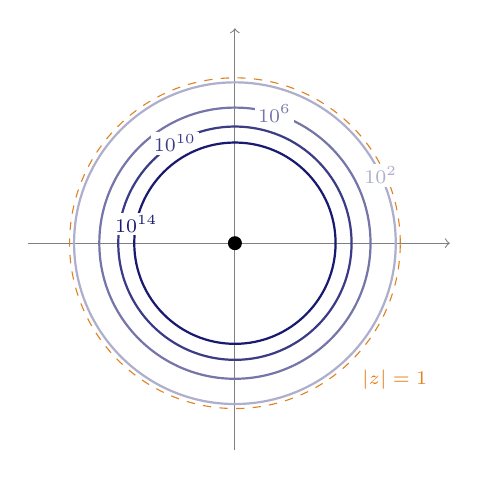
\begin{tikzpicture}[scale=2.1]
\draw[->,black!50] (-1.25,0) -- (1.3,0);
\draw[->,black!50] (0,-1.25) -- (0,1.3);
\draw[BurntOrange!90!black,dashed] (0,0) circle (1);
\draw[MidnightBlue!35,thick] (0,0) circle (0.9727);
\node[font=\scriptsize,MidnightBlue!35,fill=white,inner sep=1pt] at (0.882,0.411) {$10^{2}$};
\draw[MidnightBlue!60,thick] (0,0) circle (0.8200);
\node[font=\scriptsize,MidnightBlue!60,fill=white,inner sep=1pt] at (0.240,0.784) {$10^{6}$};
\draw[MidnightBlue!85,thick] (0,0) circle (0.7054);
\node[font=\scriptsize,MidnightBlue!85,fill=white,inner sep=1pt] at (-0.363,0.605) {$10^{10}$};
\draw[MidnightBlue,thick] (0,0) circle (0.6087);
\node[font=\scriptsize,MidnightBlue,fill=white,inner sep=1pt] at (-0.597,0.116) {$10^{14}$};
\fill (0,0) circle (1.2pt);
\node[below right,font=\scriptsize,BurntOrange!90!black] at (0.71,-0.71) {$|z|=1$};
\end{tikzpicture}
